%package list
\documentclass{article}
\usepackage[top=3cm, bottom=3cm, outer=3cm, inner=3cm]{geometry}
\usepackage{multicol}
\usepackage{graphicx}
\usepackage{url}
%\usepackage{cite}
\usepackage{hyperref}
\usepackage{array}
%\usepackage{multicol}
\newcolumntype{x}[1]{>{\centering\arraybackslash\hspace{0pt}}p{#1}}
\usepackage{natbib}
\usepackage{pdfpages}
\usepackage{multirow}
\usepackage[normalem]{ulem}
\useunder{\uline}{\ul}{}
\usepackage{svg}
\usepackage{xcolor}
\usepackage{listings}

\lstdefinestyle{ascii-tree}{
    literate={├}{|}1 {─}{--}1 {└}{+}1 
  }
\lstset{basicstyle=\ttfamily,
  showstringspaces=false,
  commentstyle=\color{red},
  keywordstyle=\color{blue}
}
%\usepackage{booktabs}
\usepackage{caption}
\usepackage{subcaption}
\usepackage{float}
\usepackage{array}

\newcolumntype{M}[1]{>{\centering\arraybackslash}m{#1}}
\newcolumntype{N}{@{}m{0pt}@{}}


%%%%%%%%%%%%%%%%%%%%%%%%%%%%%%%%%%%%%%%%%%%%%%%%%%%%%%%%%%%%%%%%%%%%%%%%%%%%
%%%%%%%%%%%%%%%%%%%%%%%%%%%%%%%%%%%%%%%%%%%%%%%%%%%%%%%%%%%%%%%%%%%%%%%%%%%%
\newcommand{\itemEmail}{jgordillome@unsa.edu.pe}
\newcommand{\itemStudent}{Jose Alonzo Gordillo Mendoza}
\newcommand{\itemCourse}{Programación Web 2}
\newcommand{\itemCourseCode}{20222083}
\newcommand{\itemSemester}{III}
\newcommand{\itemUniversity}{Universidad Nacional de San Agustín de Arequipa}
\newcommand{\itemFaculty}{Facultad de Ingeniería de Producción y Servicios}
\newcommand{\itemDepartment}{Departamento Académico de Ingeniería de Sistemas e Informática}
\newcommand{\itemSchool}{Escuela Profesional de Ingeniería de Sistemas}
\newcommand{\itemAcademic}{2023 - A}
\newcommand{\itemInput}{Del 25 Mayo 2023}
\newcommand{\itemOutput}{Al 08 Junio 2023}
\newcommand{\itemPracticeNumber}{04}
\newcommand{\itemTheme}{Python}
%%%%%%%%%%%%%%%%%%%%%%%%%%%%%%%%%%%%%%%%%%%%%%%%%%%%%%%%%%%%%%%%%%%%%%%%%%%%
%%%%%%%%%%%%%%%%%%%%%%%%%%%%%%%%%%%%%%%%%%%%%%%%%%%%%%%%%%%%%%%%%%%%%%%%%%%%

\usepackage[english,spanish]{babel}
\usepackage[utf8]{inputenc}
\AtBeginDocument{\selectlanguage{spanish}}
\renewcommand{\figurename}{Figura}
\renewcommand{\refname}{Referencias}
\renewcommand{\tablename}{Tabla} %esto no funciona cuando se usa babel
\AtBeginDocument{%
	\renewcommand\tablename{Tabla}
}

\usepackage{fancyhdr}
\pagestyle{fancy}
\fancyhf{}
\setlength{\headheight}{30pt}
\renewcommand{\headrulewidth}{1pt}
\renewcommand{\footrulewidth}{1pt}
\fancyhead[L]{\raisebox{-0.2\height}{
\includegraphics[width=3cm]{img/logo_episunsa.png}}}
\fancyhead[C]{\fontsize{7}{7}\selectfont	\itemUniversity \\ \itemFaculty \\ \itemDepartment \\ \itemSchool \\ \textbf{\itemCourse}}
\fancyhead[R]{\raisebox{-0.2\height}{
\includegraphics[width=1.2cm]{img/logo_abet}}}
\fancyfoot[L]{Estudiante Jose Gordillo Mendoza}
\fancyfoot[C]{\itemCourse}
\fancyfoot[R]{Página \thepage}

% para el codigo fuente
\usepackage{listings}
\usepackage{color, colortbl}
\definecolor{dkgreen}{rgb}{0,0.6,0}
\definecolor{gray}{rgb}{0.5,0.5,0.5}
\definecolor{mauve}{rgb}{0.58,0,0.82}
\definecolor{codebackground}{rgb}{0.95, 0.95, 0.92}
\definecolor{tablebackground}{rgb}{0.8, 0, 0}

\lstset{frame=tb,
	language=bash,
	aboveskip=3mm,
	belowskip=3mm,
	showstringspaces=false,
	columns=flexible,
	basicstyle={\small\ttfamily},
	numbers=none,
	numberstyle=\tiny\color{gray},
	keywordstyle=\color{blue},
	commentstyle=\color{dkgreen},
	stringstyle=\color{mauve},
	breaklines=true,
	breakatwhitespace=true,
	tabsize=3,
	backgroundcolor= \color{codebackground},
}

\begin{document}
	
	\vspace*{10px}
	
	\begin{center}	
		\fontsize{17}{17} \textbf{ Informe de Laboratorio \itemPracticeNumber}
	\end{center}
	\centerline{\textbf{\Large Tema: \itemTheme}}
	%\vspace*{0.5cm}	

	\begin{flushright}
		\begin{tabular}{|M{2.5cm}|N|}
			\hline 
			\rowcolor{tablebackground}
			\color{white} \textbf{Nota}  \\
			\hline 
			     \\[30pt]
			\hline 			
		\end{tabular}
	\end{flushright}	

	\begin{table}[H]
		\begin{tabular}{|x{4.7cm}|x{4.8cm}|x{4.8cm}|}
			\hline 
			\rowcolor{tablebackground}
			\color{white} \textbf{Estudiante} & \color{white}\textbf{Escuela}  & \color{white}\textbf{Asignatura}   \\
			\hline 
			{\itemStudent \par \itemEmail} & \itemSchool & {\itemCourse \par Semestre: \itemSemester \par Código: \itemCourseCode}     \\
			\hline 			
		\end{tabular}
	\end{table}		
	
	\begin{table}[H]
		\begin{tabular}{|x{4.7cm}|x{4.8cm}|x{4.8cm}|}
			\hline 
			\rowcolor{tablebackground}
			\color{white}\textbf{Laboratorio} & \color{white}\textbf{Tema}  & \color{white}\textbf{Duración}   \\
			\hline 
			\itemPracticeNumber & \itemTheme & 04 horas   \\
			\hline 
		\end{tabular}
	\end{table}
	
	\begin{table}[H]
		\begin{tabular}{|x{4.7cm}|x{4.8cm}|x{4.8cm}|}
			\hline 
			\rowcolor{tablebackground}
			\color{white}\textbf{Semestre académico} & \color{white}\textbf{Fecha de inicio}  & \color{white}\textbf{Fecha de entrega}   \\
			\hline 
			\itemAcademic & \itemInput &  \itemOutput  \\
			\hline 
		\end{tabular}
	\end{table}
	
	\section{Tarea}
	\begin{itemize}		
		\item En esta tarea usted pondrá en práctica sus conocimientos de programación en Python para dibujar un tablero de Ajedrez.
		\item La parte gráfica ya está programada, usted sólo tendrá que concentrarse en las estructuras de datos subyacentes.
		\item Con el código proporcionado usted dispondrá de varios objetos de tipo Picture para poder realizar su tarea:
	\end{itemize}
        \begin{figure}[H]
		\centering
		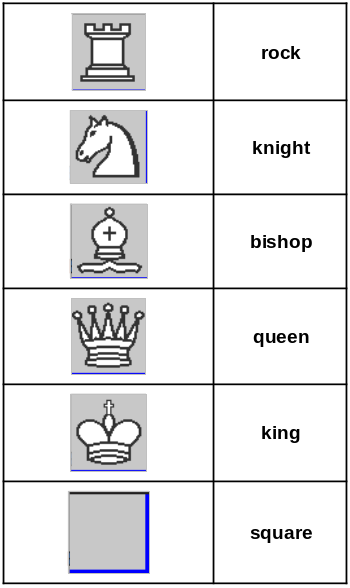
\includegraphics[width=0.25\textwidth,keepaspectratio]{img/picture.png}
	\end{figure}
 	\begin{itemize}		
            \item Estos objetos estarán disponibles importando la biblioteca: chessPictures y estarán internamente representados con arreglos de strings que podrá revisar en el archivo pieces.py
            \item La clase Picture tiene un sólo atributo: el arreglo de strings img, el cual contendrá la representación en caracteres de la figura que se desea dibujar.
            \item La clase Picture ya cuenta con una función implementada, no debe modificarla, pero si puede usarla para implementar sus otras funciones.
            \item invColor: recibe un color como un caracter de texto y devuelve su color negativo, también como texto, deberá revisar el archivo colors.py para conocer los valores negativos de cada caracter.
            \item La clase Picture contará además con varios métodos que usted deberá implementar.
            \item Tenga en cuenta que para implementar todos estos métodos, sólo deberá trabajar sobre la representación interna de un Picture, es decir su atributo img.
            \item Para dibujar una objeto Picture bastará importar el método draw de la biblioteca interpreter y usarlo de la siguiente manera.
        \end{itemize}

        \begin{lstlisting}
            python3
            Python 3.9.2 (default, Feb 28 2021, 17:03:44) 
            [GCC 10.2.1 20210110] on linux
            Type "help", "copyright", "credits" or "license" for more information.
            >>> from chessPictures import *
            >>> from interpreter import draw
            pygame 1.9.6
            Hello from the pygame community. https://www.pygame.org/contribute.html
            >>> draw(rock)
        \end{lstlisting}

        \begin{figure}[H]
		\centering
		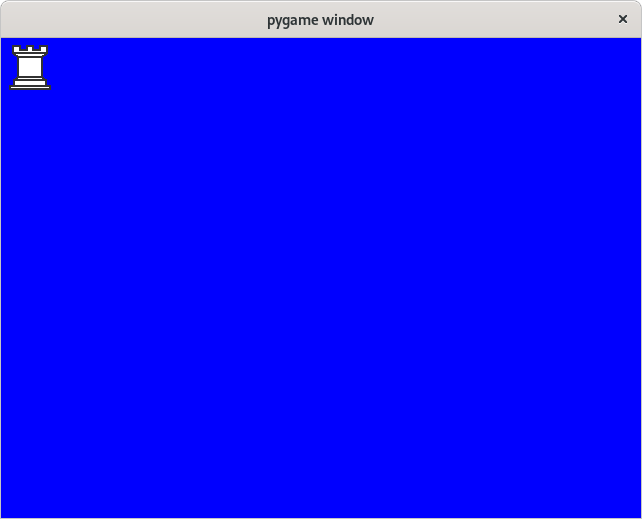
\includegraphics[width=0.7\textwidth,keepaspectratio]{img/pygame_rock.png}
	\end{figure}

	\section{URL de Repositorio Github}
	\begin{itemize}
		\item URL para el laboratorio 04 en el Repositorio GitHub.
		\item \url{https://github.com/JoseGordilloMendoza/lab04.git}
	\end{itemize}
	
	\section{Ejercicios}
 
        \subsection{Estructura de laboratorio 04}
	\begin{itemize}	
		\item El contenido que se entrega en este laboratorio es el siguiente (la carpeta latex contiene el codigo de este informe):
	\end{itemize}
	
\begin{lstlisting}[style=ascii-tree]
lab04/
    ├── chessPictures.py
    ├── colors.py
    ├── Ejercicio2.1.py
    ├── Ejercicio2.2.py
    ├── Ejercicio2.3.py
    ├── Ejercicio2.4.py
    ├── Ejercicio2.5.py
    ├── Ejercicio2.6.py
    ├── Ejercicio2.7.py
    ├── Ejercicio2.8.py
    ├── interpreter.py
    ├── picture.py
    └── pieces.py
    └── latex

\end{lstlisting}  
 
	\subsection{Implemente los métodos de la clase Picture. Se recomienda que implemente la clase picture por etapas, probando realizar los dibujos que se muestran en la siguiente preguntas.}
 
        \begin{itemize}	
		\item Primero explicaremos la \textbf{class Picture:} 
	\end{itemize}
 
	\begin{lstlisting}[language=bash,caption={Importación de módulos}][H]
            from colors import *
	\end{lstlisting}
        En este grupo, se importa el módulo colors. Esto significa que se está utilizando un archivo llamado colors.py que contiene definiciones de colores. Probablemente, el módulo proporciona una funcionalidad para trabajar con colores en el código.
                  
	\begin{lstlisting}[language=bash,caption={Definición de la clase Picture}][H]
            class Picture:
              def __init__(self, img):
                self.img = img;
	\end{lstlisting}
En este grupo, se define la clase Picture, que representa una imagen o figura. La clase tiene un constructor \_\_init\_\_ que recibe un parámetro img y asigna ese valor al atributo img de la instancia.

        \begin{lstlisting}[language=bash,caption={Métodos de la clase Picture para manipulación de imágenes}][H]
              def __eq__(self, other):
                return self.img == other.img
            
              def _invColor(self, color):
                if color not in inverter:
                  return color
                return inverter[color]
            
              def verticalMirror(self):
                vertical = []
                vertical = self.img[::-1]
                return Picture(vertical)
            
              def horizontalMirror(self):
                length = len(self.img[0])
                newimg = []
            
                for r in self.img:
                  row = ""
                  x = 0
                  while x < length:
                    row += r[length -1 -x]
                    x += 1
                  newimg.append(row)
            
                return Picture(newimg)
            
              def negative(self):
                newimg = []
            
                for r in self.img:
                  x = 0
                  row = ""
                  while x < len(r):
                    row += self._invColor(r[x])
                    x += 1
                  newimg.append(row)
            
                return Picture(newimg)
            
              def join(self, p):
                newimg = []
                x = 0
                while x < len(self.img):
                  newimg.append(self.img[x] + p.img[x])
                  x += 1
            
                return Picture(newimg)
            
              def up(self, p):
                newimg = []
                for r in self.img:
                  newimg.append(r)
            
                for r in p.img:
                  newimg.append(r)
                return Picture(newimg)
            
              def under(self, p):
                newimg = []
                for r in p.img:
                  newimg.append(r)
            
                for r in self.img:
                  newimg.append(r)
            
                return Picture(newimg)
            
              def horizontalRepeat(self, n):
                newimg = []
            
                for r in self.img:
                  x = 1
                  row = ""
                  while x <= n:
                    row += r
                    x += 1
                  newimg.append(row)
            
                return Picture(newimg)
            
              def verticalRepeat(self, n):
                newimg = []
            
                x = 1
                while x <= n:
                  for r in self.img:
                    newimg.append(r)
                  x += 1
            
                return Picture(newimg)
            
              def rotate(self):
                newimg = []
                i = 0
                while (i < len(self.img[0])):
                  row = ""
                  j = len(self.img) - 1
                  while (j >= 0):
                    aux = self.img[j]
                    row += aux[i]
                    j -= 1
                  newimg.append(row)
                  i += 1
            
                return Picture(newimg)
            
              def setBackground(self, p):
                backgroundColor = p.img[0][0]
                newimg = []
                for r in self.img:
                  x = 0
                  row = ""
                  while x < len(r):
                    if r[x] == " ":
                      row += backgroundColor
                    else:
                      row += r[x]
                    x += 1
                  newimg.append(row)
            
                return Picture(newimg)
	\end{lstlisting}
Este código define una clase llamada "Picture" que representa una imagen como una lista de cadenas de caracteres. La clase tiene métodos para realizar diferentes operaciones en imágenes. El método "eq" compara si dos imágenes son iguales. El método "\_invColor" invierte el color de un píxel. Los métodos "verticalMirror" y "horizontalMirror" reflejan vertical y horizontalmente la imagen original. El método "negative" crea una nueva imagen aplicando el inverso de color a cada píxel. Los métodos "join", "up" y "under" combinan imágenes concatenando filas en diferentes configuraciones. Los métodos "horizontalRepeat" y "verticalRepeat" repiten la imagen original horizontal y verticalmente. El método "rotate" rota la imagen en sentido horario. El método "setBackground" establece el color de fondo de la imagen, setteando un fondo.

        \begin{lstlisting}[language=bash,caption={Método \_invColor}][H]
              def _invColor(self, color):
                if color not in inverter:
                  return color
                return inverter[color]
	\end{lstlisting}
Este grupo contiene el método privado \_invColor que se utiliza para invertir un color. Verifica si el color está definido en el módulo inverter y, de ser así, devuelve el color invertido.

        \begin{lstlisting}[language=bash,caption={Método rotate}][H]
              def rotate(self):
                newimg = []
                i = 0
                while (i < len(self.img[0])):
                  row = ""
                  j = len(self.img) - 1
                  while (j >= 0):
                    aux = self.img[j]
                    row += aux[i]
                    j -= 1
                  newimg.append(row)
                  i += 1
            
                return Picture(newimg)
	\end{lstlisting}
Este grupo contiene el método rotate que rota la imagen 90 grados. Crea una nueva imagen newimg y realiza una rotación de cada píxel de la imagen original, moviendo las columnas a las filas en newimg.

        \begin{lstlisting}[language=bash,caption={Método setBackground}][H]
              def setBackground(self, p):
                backgroundColor = p.img[0][0]
                newimg = []
                for r in self.img:
                  x = 0
                  row = ""
                  while x < len(r):
                    if r[x] == " ":
                      row += backgroundColor
                    else:
                      row += r[x]
                    x += 1
                  newimg.append(row)
            
                return Picture(newimg)
	\end{lstlisting}
Este grupo contiene el método setBackground que establece el color de fondo de la imagen utilizando el primer carácter de la primera fila de p.img. Crea una nueva imagen newimg y reemplaza los espacios en blanco en self.img con el color de fondo.

	\begin{itemize}	
		\item La siguiente clase es \textbf{class Interpreter:} 
	\end{itemize}
	\begin{lstlisting}[language=bash,caption={Importación de módulos y definición de la función parseLine}][H]
            import pygame, sys
            from pygame.locals import *
            from colors import *
            
            def parseLine(DISPLAY, y, s):
              x = 0
              for c in s:
                pygame.draw.line(DISPLAY, color[c], (x, y), (x, y))
                x += 1
	\end{lstlisting}
En este grupo, se importan los módulos necesarios para utilizar la biblioteca Pygame y el módulo colors. Pygame es una biblioteca popular para el desarrollo de juegos y aplicaciones multimedia en Python. Además, se define la función parseLine, que se utiliza para dibujar una línea en la ventana de visualización.	

	\begin{lstlisting}[language=bash,caption={Definición de la función draw}][H]
            def draw(picture):
              try:
                img = picture.img
              except:
                img = picture
              pygame.init()
            
              DISPLAY=pygame.display.set_mode((640, 480))
              DISPLAY.fill(BLUE)
            
              n = len(img)
              for i in range(0, n):
                parseLine(DISPLAY, i, img[i])
            
              while True:
                for event in pygame.event.get():
                  if event.type==QUIT:
                    pygame.quit()
                pygame.display.update()
	\end{lstlisting}
En este grupo, se define la función principal draw que se utiliza para dibujar la imagen en una ventana. La función toma un argumento picture, que puede ser una instancia de la clase Picture o simplemente una matriz de imagen. El código realiza las siguientes acciones:Intenta obtener la matriz de imagen img de picture.img. Si picture no tiene el atributo img, asume que picture ya es la matriz de imagen.Inicializa Pygame.Crea una ventana de visualización de tamaño 640x480 y la rellena con el color BLUE.Obtiene la longitud n de la matriz de imagen img.Itera sobre las líneas de la imagen y llama a la función parseLine para dibujar cada línea en la ventana de visualización.En un bucle infinito, maneja los eventos de Pygame. Si se detecta un evento de cierre de la ventana, finaliza el programa Pygame y cierra la ventana.Actualiza la ventana de visualización para mostrar los cambios.

	\begin{lstlisting}[language=bash,caption={Línea final de código}][H]
            pygame.display.update()
	\end{lstlisting}
Esta línea de código actualiza la ventana de visualización para mostrar los cambios realizados.

\begin{itemize}	
		\item La siguiente clase es \textbf{class Colors:} 
	\end{itemize}
 
	\begin{lstlisting}[language=bash,caption={Clase Color}][H]
            # Definir constantes para representar colores en formato RGB
            WHITE = (255, 255, 255)
            BLACK = (0, 0, 0)
            LIGHTGRAY = (200, 200, 200)
            GRAY = (127, 127, 127)
            DARKGRAY = (50, 50, 50)
            BLUE = (0, 0, 255)
            
            # Definir un diccionario llamado "color" para mapear símbolos a colores
            color = {
              '_': LIGHTGRAY,  # Símbolo '_' representa el color LIGHTGRAY
              '=': GRAY,       # Símbolo '=' representa el color GRAY
              '.': WHITE,      # Símbolo '.' representa el color WHITE
              '@': BLACK,      # Símbolo '@' representa el color BLACK
              '#': DARKGRAY,   # Símbolo '#' representa el color DARKGRAY
              ' ': BLUE,       # Símbolo ' ' representa el color BLUE
            }
            
            # Definir un diccionario llamado "inverter" para mapear símbolos a sus inversos
            inverter = {
              '_': '=',   # Símbolo '_' tiene el inverso '='
              '=': '_',   # Símbolo '=' tiene el inverso '_'
              '.': '@',   # Símbolo '.' tiene el inverso '@'
              '@': '.',   # Símbolo '@' tiene el inverso '.'
            }
	\end{lstlisting}
Este código define constantes que representan colores en formato RGB, como blanco, negro, gris claro, gris, gris oscuro y azul. También define dos diccionarios: "color" que mapea símbolos a colores y "inverter" que mapea símbolos a sus inversos. Por ejemplo, el símbolo \'\_' representa el color gris claro y su inverso es el símbolo '=', el símbolo '.' representa el color blanco y su inverso es el símbolo '@', y así sucesivamente. Estos diccionarios pueden utilizarse para asignar colores a símbolos en un contexto específico.

 \clearpage

\begin{itemize}	
		\item La siguiente clase es \textbf{class chessPictures:} 
	\end{itemize}
	\begin{lstlisting}[language=bash,caption={Creación de objetos Picture para el alfil, el rey, el caballo, el peón, la reina y la torre}][H]
            # Importar los módulos "pieces" y "picture"
            from pieces import *
            from picture import *
            
            # Crear un objeto "Picture" para representar un alfil y asignarlo a la variable "elAlfil"
            elAlfil = Picture(BISHOP)
            
            # Crear un objeto "Picture" para representar un rey y asignarlo a la variable "elRey"
            elRey = Picture(KING)
            
            # Crear un objeto "Picture" para representar un caballo y asignarlo a la variable "elCaballo"
            elCaballo = Picture(KNIGHT)
            
            # Crear un objeto "Picture" para representar un peón y asignarlo a la variable "elPeon"
            elPeon = Picture(PAWN)
            
            # Crear un objeto "Picture" para representar una reina y asignarlo a la variable "laReina"
            laReina = Picture(QUEEN)
            
            # Crear un objeto "Picture" para representar una torre y asignarlo a la variable "laTorre"
            laTorre = Picture(ROCK)
            
            # Crear un objeto "Picture" para representar un cuadrado y asignarlo a la variable "cuadrado"
            cuadrado = Picture(SQUARE)
	\end{lstlisting}
El código comienza importando los módulos "pieces" y "picture" que contienen definiciones y variables relacionadas con piezas de ajedrez y representación de imágenes. Luego, se crean varios objetos de la clase "Picture" para representar diferentes piezas de ajedrez, como el alfil, el rey, el caballo, el peón, la reina y la torre. Cada objeto se asigna a una variable específica, lo que permite acceder a ellos más tarde. Además, se crea un objeto "Picture" adicional para representar un cuadrado. Estos objetos se crean utilizando las variables importadas del módulo "pieces", que contienen representaciones de texto de las piezas de ajedrez. En resumen, el código establece variables con imágenes predefinidas de piezas de ajedrez y un cuadrado, lo que facilita su uso posterior en la manipulación y visualización de imágenes relacionadas con el ajedrez.

\clearpage
	\begin{itemize}	
		\item La siguiente clase es \textbf{class Ejercicio2.1:} 
	\end{itemize}
 
	\begin{lstlisting}[language=bash,caption={\textbf{PRIMER EJERCICIO}}][H]
            from interpreter import draw
            from chessPictures import *
            
            # Crear la primera línea como la unión del caballo y su negativo
            line1 = elCaballo.join(elCaballo.negative())
            
            # Crear la segunda línea como la unión del negativo del caballo y el caballo original
            line2 = elCaballo.negative().join(elCaballo)
            
            # Combinar las dos líneas en una figura
            figure = line1.up(line2)
            
            # Dibujar la figura
            draw(figure)
	\end{lstlisting}
En esta parte tenemos la importacion del interprete especificando el "draw" y todo de "chessPictures", entonces en la linea se combina un caballo normal y a su derecha su negativo, en la segunda ocurre lo contrario, el negativo a su derecha uno normal, luego los unimos, la linea 1 sobre la linea 2 y lo dibujamos finalmente.

\begin{itemize}	
		\item La siguiente clase es \textbf{class Ejercicio2.2:} 
	\end{itemize}
 
	\begin{lstlisting}[language=bash,caption={\textbf{SEGUNDO EJERCICIO}}][H]
            from interpreter import draw
            from chessPictures import *
            
            # Crear la primera línea como la unión del caballo y su negativo
            line1 = elCaballo.join(elCaballo.negative())
            
            # Crear la segunda línea como la línea 1 reflejada horizontalmente
            line2 = line1.horizontalMirror()
            
            # Combinar las dos líneas en una figura
            figure = line1.up(line2)
            
            # Dibujar la figura
            draw(figure)
	\end{lstlisting}
En este código, se importa la función draw del módulo interpreter y las variables del módulo chessPictures. Luego, se crea una figura compuesta por dos líneas: la primera línea es la unión del objeto elCaballo con su negativo, y la segunda línea es la primera línea reflejada horizontalmente. Estas dos líneas se combinan utilizando los métodos up() y join() de la clase Picture. Finalmente, la figura resultante se dibuja en una ventana de visualización llamando a la función draw.En resumen dibujamos la linea 1 y la unimos con la linea 2 que es su reflejo horizontal, la linea 1 esta encima de la linea 2.

\begin{itemize}	
		\item La siguiente clase es \textbf{class Ejercicio2.3:} 
	\end{itemize}
 
	\begin{lstlisting}[language=bash,caption={\textbf{TERCER EJERCICIO}}][H]
            from interpreter import draw
            from chessPictures import *
            
            # Crear una figura compuesta por la repetición horizontal de la imagen de la reina
            figure = laReina.horizontalRepeat(4)
            
            # Dibujar la figura
            draw(figure)
	\end{lstlisting}
En este código, se importa la función draw del módulo interpreter y las variables del módulo chessPictures. A continuación, se crea una figura compuesta por la repetición horizontal de la imagen de la reina, utilizando el método horizontalRepeat(). Esta repeticion se da 4 veces, por lo que son 4 reinas normales.

\begin{itemize}	
		\item La siguiente clase es \textbf{class Ejercicio2.4:} 
	\end{itemize}
 
	\begin{lstlisting}[language=bash,caption={\textbf{CUARTO EJERCICIO}}][H]
            from interpreter import draw
            from chessPictures import *
            
            # Crear la base del patrón (un cuadro blanco seguido de un cuadro negro)
            base = cuadrado.join(cuadrado.negative())
            
            # Crear una figura compuesta por la repetición horizontal de la base
            figure = base.horizontalRepeat(4)
            
            # Dibujar la figura
            draw(figure)
	\end{lstlisting}
En este código, se importa la función draw del módulo interpreter y se importan las variables del módulo chessPictures. Luego, se crea una base para el patrón uniendo un cuadro blanco con un cuadro negro utilizando los métodos join() y negative() de la clase Picture. A continuación, se genera una figura compuesta por la repetición horizontal de la base utilizando el método horizontalRepeat(). Lo que en sintesis es 2 cuadrados (normal y negativo) repetidas horizontalmente 4 veces.

\begin{itemize}	
		\item La siguiente clase es \textbf{class Ejercicio2.5:} 
	\end{itemize}
 
	\begin{lstlisting}[language=bash,caption={\textbf{QUINTO EJERCICIO}}][H]
            from interpreter import draw
            from chessPictures import *
            
            # Crear la base del tablero (un cuadro blanco seguido de un cuadro negro)
            base = cuadrado.join(cuadrado.negative())
            negativeBase = base.negative()
            
            # Crear una figura compuesta por la repetición horizontal del negativo de la base
            figure = negativeBase.horizontalRepeat(4)
            
            # Dibujar la figura
            draw(figure)
	\end{lstlisting}
Se genera una figura compuesta por la repetición horizontal del negativo de la base utilizando el método horizontalRepeat(). Finalmente, se muestra la figura en una ventana de visualización llamando a la función draw(). En resumen, se muestra una imagen que representa un tablero de ajedrez con cuadros negros y blancos alternados, pero con los colores invertidos.

\begin{itemize}	
		\item La siguiente clase es \textbf{class Ejercicio2.6:} 
	\end{itemize}
 
	\begin{lstlisting}[language=bash,caption={\textbf{SEXTO EJERCICIO}}][H]
            from interpreter import draw
            from chessPictures import *
            
            # Crear la base del tablero (un cuadro negro seguido de un cuadro blanco)
            base = cuadrado.join(cuadrado.negative())
            negativeBase = base.negative()
            
            # Crear una fila del tablero
            row = base.horizontalRepeat(4)
            negativeRow = negativeBase.horizontalRepeat(4)
            
            # Combinar las filas en pares, alternando entre una fila y su negativo
            rowPair = row.up(negativeRow)
            
            # Crear una figura compuesta por las filas repetidas verticalmente
            figure = rowPair.verticalRepeat(2)
            
            # Dibujar la figura
            draw(figure)
	\end{lstlisting}
Este programa dibuja un tablero de ajedrez en una ventana de visualización. Primero, se crea la base del tablero mediante la unión de un cuadro negro y un cuadro blanco utilizando el método join() y el método negative() de la clase Picture. Luego, se genera una fila del tablero mediante la repetición horizontal de la base. Posteriormente, se combinan las filas en pares alternando entre una fila y su negativo utilizando los métodos up() y horizontalRepeat(). A continuación, se crea una figura compuesta por la repetición vertical de los pares de filas utilizando el método verticalRepeat(). Finalmente, se muestra la figura resultante en una ventana de visualización llamando a la función draw(). En resumen, el programa crea y muestra un tablero de ajedrez con cuadros negros y blancos alternados.

\begin{itemize}	
		\item La siguiente clase es \textbf{class Ejercicio2.7:} 
	\end{itemize}
 
	\begin{lstlisting}[language=bash,caption={\textbf{SEPTIMO EJERCICIO}: Creación de imágenes de piezas negras}][H]
            # Crear una imagen del cuadro negro
            negativeSquare = cuadrado.negative()
            
            # Crear imágenes de las piezas negras y establecer el fondo adecuado
            torreNegra1 = laTorre.negative().setBackground(cuadrado)
            caballoNegro1 = elCaballo.negative().setBackground(negativeSquare)
            alfilNegro1 = elAlfil.negative().setBackground(cuadrado)
            reynaNegra = laReina.negative().setBackground(negativeSquare)
            reyNegro = elRey.negative().setBackground(cuadrado)
            alfilNegro2 = elAlfil.negative().setBackground(negativeSquare)
            caballoNegro2 = elCaballo.negative().setBackground(cuadrado)
            torreNegra2 = laTorre.negative().setBackground(negativeSquare)
	\end{lstlisting}
En el primer grupo, se crean las imágenes de las piezas negras del ajedrez. Se utiliza el método negative() para obtener las versiones negativas de las imágenes de las piezas y se establece el fondo adecuado utilizando el método setBackground(). Se crean las imágenes de la torre negra, el caballo negro, el alfil negro, la reina negra, el rey negro y se repiten las imágenes del alfil negro y el caballo negro.

	\begin{lstlisting}[language=bash,caption={\textbf{SEPTIMO EJERCICIO}: Creación de filas de piezas negras y peones negros}][H]
            # Crear una fila de las piezas negras
            row1 = torreNegra1.join(caballoNegro1).join(alfilNegro1).join(reynaNegra).join(reyNegro).join(alfilNegro2).join(caballoNegro2).join(torreNegra1)
            
            # Crear un par de peones negros
            coupleBlackPawn = elPeon.negative().setBackground(negativeSquare).join(elPeon.negative().setBackground(cuadrado))
            
            # Crear una segunda fila de los peones negros
            row2 = coupleBlackPawn.horizontalRepeat(4)
	\end{lstlisting}
En el segundo grupo, se crean una fila de las piezas negras y un par de peones negros. Se utiliza el método join() para unir las imágenes de las piezas en una fila. Además, se repite horizontalmente el par de peones negros.

	\begin{lstlisting}[language=bash,caption={\textbf{SEPTIMO EJERCICIO}: Creación del tablero completo}][H]
            # Crear una base del tablero
            base = cuadrado.join(cuadrado.negative())
            negativeBase = base.negative()
            
            # Crear una fila del tablero
            row = base.horizontalRepeat(4)
            negativeRow = negativeBase.horizontalRepeat(4)
            
            # Combinar las filas de manera alternada
            rowPair = row.up(negativeRow)
            
            # Crear las filas 3 a 6 del tablero
            row3_6 = rowPair.verticalRepeat(2)
            
            # Crear la séptima fila del tablero
            row7 = row2.negative()
            
            # Crear la octava fila del tablero
            row8 = row1.negative()
            
            # Dibujar el tablero completo
            draw(row1.up(row2).up(row3_6).up(row7).up(row8))
            
	\end{lstlisting}
En el tercer grupo, se crea la base del tablero y se generan las filas del tablero mediante repeticiones y combinaciones. Se combinan las filas de manera alternada utilizando el método up(), y se generan las filas 3 a 6 del tablero mediante el método verticalRepeat(). Luego, se crean la séptima y octava fila del tablero invirtiendo las filas anteriores. Finalmente, se dibuja el tablero completo llamando a la función draw() y pasando las filas correspondientes.

\begin{itemize}	
		\item La siguiente clase es \textbf{class Ejercicio2.8:} 
	\end{itemize}
 
	\begin{lstlisting}[language=bash,caption={\textbf{OCTAVO EJERCICIO}}][H]
            from interpreter import draw
            from chessPictures import *
            
            # Llama a la función draw y pasa como argumento la composición de la imagen del
            # espejo vertical del caballo (elCaballo.verticalMirror()) y la imagen rotada del
            # caballo (elCaballo.rotate())
            draw(elCaballo.verticalMirror().join(elCaballo.rotate()))
	\end{lstlisting}
Este código llama a la función draw() y pasa como argumento la composición de dos imágenes del caballo. La primera imagen es el espejo vertical del caballo, obtenido mediante el método verticalMirror() aplicado a elCaballo. La segunda imagen es la imagen rotada del caballo, obtenida mediante el método rotate() aplicado a elCaballo. Estas dos imágenes se unen utilizando el método join(). Finalmente, la composición resultante se pasa como argumento a la función draw() para ser dibujada.

\section{Cuestionario}
	\begin{itemize}
		\item \textbf{¿Qué son los archivos *.pyc?}
  \newline
Los archivos .pyc son archivos de bytecode generados por Python cuando se compila un archivo fuente de Python (.py). El bytecode es una representación intermedia del código fuente de Python que es interpretada por la máquina virtual de Python (PVM) para ejecutar el programa.
Cuando se ejecuta un archivo de Python, el intérprete de Python compila el código fuente a bytecode y luego lo ejecuta. Durante el proceso de compilación, se genera un archivo *.pyc que contiene el bytecode compilado. Este archivo *.pyc se guarda en el mismo directorio que el archivo fuente *.py.
		\item \textbf{¿Para qué sirve el directorio pycache?}
  \newline
  El directorio pycache es un directorio especial que se crea automáticamente en Python 3.x para almacenar archivos de código compilado (archivos .pyc) y metadatos relacionados. Estos archivos .pyc contienen el código fuente de Python compilado en formato de bytecode, que es más rápido de ejecutar que el código fuente en sí.
  Por tanto decimos que es utilizado por Python para almacenar archivos de código compilado y optimizar el tiempo de carga y ejecución de módulos importados en un proyecto.
		\item \textbf{¿Cuáles son los usos y lo que representa el subguión en Python?}
  \newline
  El subguión en Python tiene varios usos y representaciones, dependiendo del contexto en el que se utilice. Aquí hay algunos casos comunes:
    - Variable temporal: En muchas ocasiones, el subguión se utiliza como una variable temporal o de descarte cuando no es relevante el valor en sí. Por ejemplo, en un bucle for, si solo nos interesa el índice y no el valor en sí, podemos usar como una convención para indicar que el valor no se utilizará.\newline
    - Ignorar valores de retorno: Cuando una función devuelve múltiples valores y solo nos interesan algunos de ellos, podemos utilizar el subguión para ignorar los valores no deseados. Esto se conoce como "desempaquetado parcial".\newline
    - Traducción o internacionalización: En el contexto de la internacionalización y la traducción de cadenas de texto, el subguiónse utiliza como una convención para marcar cadenas de texto que deben ser traducidas. Es común verlo en bibliotecas y aplicaciones que admiten múltiples idiomas.\newline
    - Módulo especial: Existe un módulo especial llamado, que se utiliza para traducir cadenas de texto en aplicaciones internacionales. Este módulo permite definir las traducciones para diferentes idiomas y acceder a ellas mediante la función ().
	\end{itemize}	
 \section{Conclusiones}
	\begin{itemize}
		\item Python es un lenguaje de programación versátil y poderoso que se utiliza en una amplia variedad de aplicaciones, desde desarrollo web y científico hasta automatización de tareas y aprendizaje automático.
		\item Python cuenta con una amplia variedad de bibliotecas y frameworks que permiten ampliar sus funcionalidades y acelerar el desarrollo de aplicaciones. Algunas bibliotecas populares incluyen NumPy, Pandas, Matplotlib, Django y Flask.
		\item Python es un lenguaje multiplataforma, lo que significa que podemos escribir código en Python y ejecutarlo en diferentes sistemas operativos, como Windows, macOS y Linux.
            \item Python se destaca por su sintaxis clara y legible, lo que facilita la lectura y comprensión del código. Esto lo convierte en un lenguaje ideal tanto para principiantes como para programadores experimentados.
	\end{itemize}	
\clearpage

\section{Referencias}
\begin{itemize}			
	\item \url{https://www.w3schools.com/python/}
        \item \url{https://docs.python.org/3/tutorial/}
\end{itemize}	
	
%\clearpage
%\bibliographystyle{apalike}
%\bibliographystyle{IEEEtranN}
%\bibliography{bibliography}
			
\end{document}
